% Figure 3: schematic of the two guarantees (no data; illustration only).
% (a) Theorem A: the logit margin M(x) of the mean predictor certifies an l2 ball
%     of radius r(x) = M(x)/(sqrt(2) L) around x.
% (b) Proposition 2: a single-path flip needs either a clean path margin G(x)
%     within beta of the boundary, or a path movement of at least beta.
\documentclass[border=4pt]{standalone}
\usepackage{times}
\usepackage{amsmath,amssymb}
\usepackage{pgfplots}
\pgfplotsset{compat=1.17}
\usetikzlibrary{arrows.meta,decorations.pathreplacing,calc}
\begin{document}
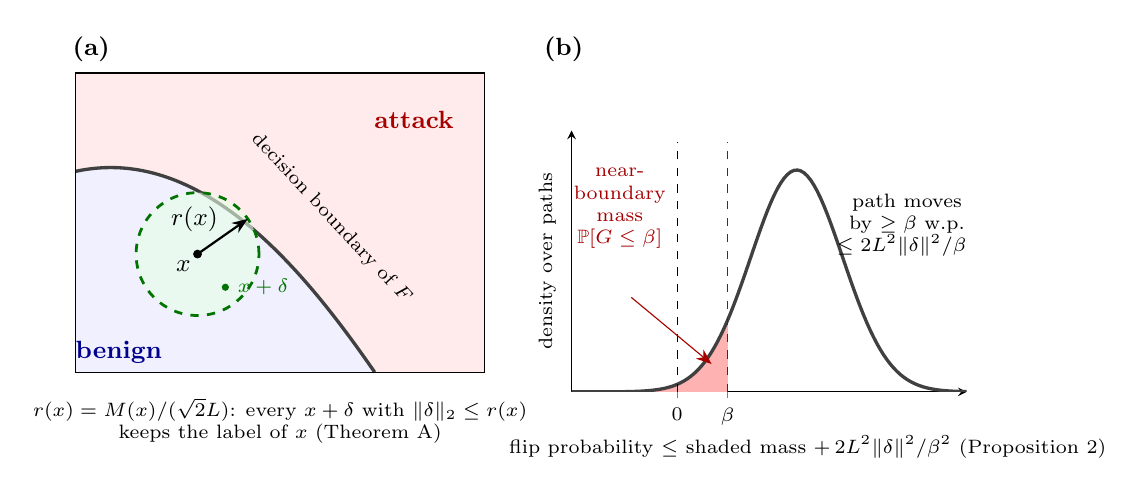
\begin{tikzpicture}[font=\small]
%% ---------------- (a) certified ball ----------------
\begin{scope}
\fill[blue!6] (0,0) rectangle (5.2,3.8);
\fill[red!8] (0,3.8) -- (0,2.55) .. controls (1.6,2.9) and (2.9,1.3) .. (3.8,0) -- (5.2,0) -- (5.2,3.8) -- cycle;
\draw[line width=1.2pt, black!75] (0,2.55) .. controls (1.6,2.9) and (2.9,1.3) .. (3.8,0);
\node[blue!55!black, font=\small\bfseries] at (0.55,0.25) {benign};
\node[red!65!black, font=\small\bfseries] at (4.3,3.2) {attack};
\node[font=\scriptsize, rotate=-47] at (3.25,1.95) {decision boundary of $F$};
\coordinate (x) at (1.55,1.5);
\draw[dashed, line width=1pt, green!45!black, fill=green!10, fill opacity=0.6] (x) circle (0.78);
\fill (x) circle (1.6pt) node[below left=-1pt] {$x$};
\draw[-{Stealth[length=2mm]}, line width=0.8pt] (x) -- ++(35:0.78) node[midway, above left=-2pt] {$r(x)$};
\coordinate (xd) at ($(x)+(-50:0.55)$);
\fill[green!45!black] (xd) circle (1.3pt) node[right=1pt, font=\scriptsize] {$x+\delta$};
\node[align=center, font=\scriptsize, fill=white, rounded corners=2pt, inner sep=2pt] at (2.6,-0.62)
  {$r(x)=M(x)/(\sqrt2L)$: every $x+\delta$ with $\|\delta\|_2\le r(x)$\\ keeps the label of $x$ (Theorem A)};
\node[font=\small\bfseries] at (0.2,4.1) {(a)};
\draw (0,0) rectangle (5.2,3.8);
\end{scope}
%% ---------------- (b) path-wise margin distribution ----------------
\begin{scope}[xshift=6.3cm]
\begin{axis}[
  width=6.6cm, height=4.9cm, at={(0,-0.25cm)},
  xmin=-2.3, xmax=6.3, ymin=0, ymax=0.47,
  axis lines=left, ytick=\empty, xtick={0,1.1}, xticklabels={$0$,$\beta$},
  xlabel={clean path margin $G(x)$}, ylabel={density over paths},
  label style={font=\scriptsize}, tick label style={font=\scriptsize},
  samples=120, domain=-2.3:6.3,
]
\addplot[draw=none, fill=red!30, domain=-2.3:1.1] {exp(-(x-2.6)^2/(2*1.0^2))/(sqrt(2*pi)*1.0)} \closedcycle;
\addplot[line width=1.2pt, black!75] {exp(-(x-2.6)^2/(2*1.0^2))/(sqrt(2*pi)*1.0)};
\draw[dashed] (axis cs:0,0) -- (axis cs:0,0.45);
\draw[dashed, red!65!black] (axis cs:1.1,0) -- (axis cs:1.1,0.45);
\node[font=\scriptsize, red!65!black, align=center] at (axis cs:-1.25,0.33) {near-\\boundary\\ mass\\ $\mathbb P[G\le\beta]$};
\draw[-{Stealth[length=2mm]}, red!65!black] (axis cs:-1.0,0.17) -- (axis cs:0.75,0.05);
\node[font=\scriptsize, align=center] at (axis cs:5.0,0.3) {path moves\\ by $\ge\beta$ w.p.\\ $\le 2L^2\|\delta\|^2/\beta^2$};
\end{axis}
\node[font=\small\bfseries] at (-0.1,4.1) {(b)};
\node[align=center, font=\scriptsize, fill=white, inner sep=2pt] at (3.0,-0.95)
  {flip probability $\le$ shaded mass $+\,2L^2\|\delta\|^2/\beta^2$ (Proposition 2)};
\end{scope}
\end{tikzpicture}
\end{document}
